\documentclass[11pt,a4paper]{article}
%\usepackage{beamerarticle}

%\usefonttheme[onlymath]{serif}
\usepackage[ngerman]{babel}
\usepackage[utf8]{inputenc}
\usepackage[T1]{fontenc}
\usepackage{tikz}
\usetikzlibrary{positioning, arrows}
\usepackage{listings}
\usepackage{fancybox}
\usepackage{color}
\usepackage{hyperref}
\usepackage{fancyhdr}
\usepackage{pifont}% http://ctan.org/pkg/pifont
\newcommand{\cmark}{\ding{51}}%
\newcommand{\xmark}{\ding{55}}%
\pagestyle{fancy}
\lhead{\today}
\rhead{Formatiert von: PP}
\chead{Gruppe: swp15.gkp}
%\cfoot{center of the footer!}
\renewcommand{\headrulewidth}{0.8pt}
%\renewcommand{\footrulewidth}{0.4pt}
\begin{document}
\center {\huge Arbeitsplan}
\flushleft
\tableofcontents
\section{Projektvision}

/LV10/ Als Spieler will ich Pacman auf einen
realen Kartenausschnitt spielen.\\


\subsection{Ziele}

/LZ10/ Als Spieler möchte ich, dass die
Spielewelt ein Overlay von einer realen Karte
ist. \\
/LZ20/ Als Spieler möchte ich mit anderen
Spielern zusammen spielen können.\\
/LZ30/ Als Spieler möchte ich meine
Highscores mit denen anderer vegleichen.\\

\subsection{Rahmenbedingungen} 

/LR10/ Zielgruppe sind Menschen auf aller
Welt die ein paar Minuten Ablenkung
brauchen.\\
/LR20/ Dieses Projekt wird ein Browsergame.\\

\subsection{Kontext und Überblick}

/LK10/ Als Spieler möchte ich das Spiel ohne
Installation spielen können.\\

\subsection{Qualitätsanforderungen}

/LQE10/ Als Spieler will ich Levels spielen,
die der Topologie der originalen Pacman
Levels möglichst nahe kommen.\\

\section{Vorraussetzungen}

Unser Projekt baut auf kein bereits vorhandenes Projekt auf, es existieren allerdings bereits
verschiedene Umsetzungen des Spielkonzepts, die erweitert werden können. Als technische
Voraussetzungen werden Standartwebtechnologien wie HTML oder JavaScript benötigt, welche vom
Server ausgeliefert und vom Browser des Spielers interpretiert werden. Außerdem muss der Browser
auch Daten von einem SPARQL-Endpoint extrahieren können um die Kartendaten zu erhalten.
Es wird also ein Webserver mit ausreichend Speicherplatz für Website und Spiel und eventuell
gespeicherte Kartendaten benötigt, zudem auch einen SPARQL-Endpoint von dem Geo- und
Metadaten extrahieren kann und ein Client der einen Webbrowser besitzt der in der Lage ist die
Webseite sowie das Spiel anzuzeigen.

\clearpage
\section{Designübersicht und Funktionalität}
\begin{figure}[htb]
  \centering
  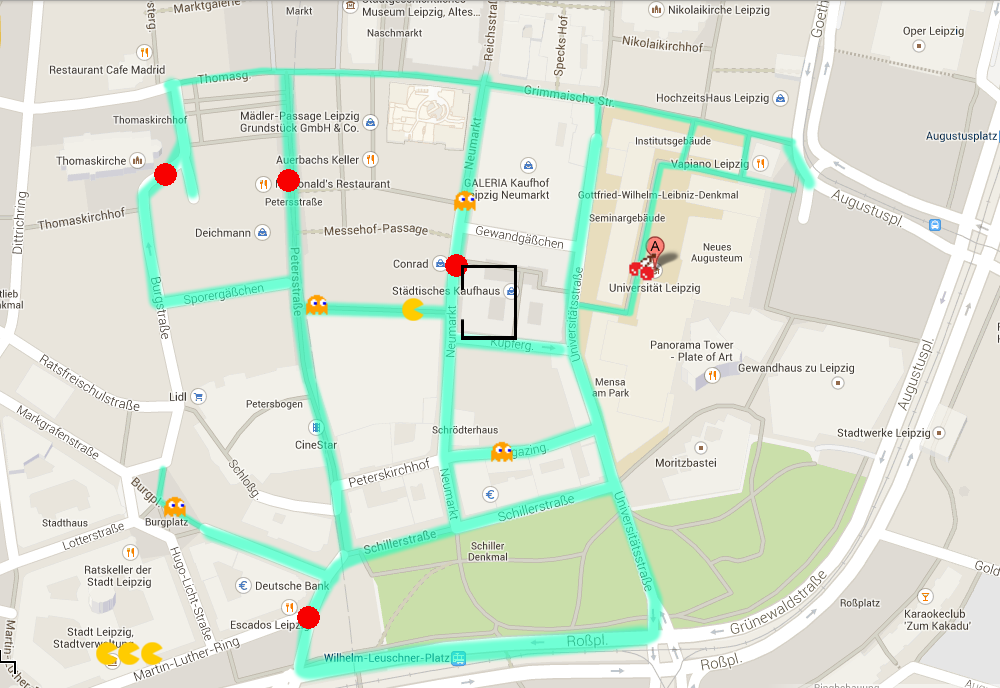
\includegraphics[scale=0.3]{pacman.png}
%\caption{hier wird anhand von code gezeigt auf welchen Standard wir uns geeinigt haben}
  \label{PNFs}
\end{figure} 

Zu erstellen sind die folgenden Komponenten: Die Spielelogik, ein Datenbanksystem zum Speichern der Highscores und ein Kartenmodul. Aufgabe des Kartenmodules ist es aus den Realdaten einer Kartenapi einen Graphen als Grundlage für Pacman Level zu erstellen und dieses Level mit Spielelementen analog zu semantischen Informationen zu Orten anzureichern. Interagieren kann der Nutzer mit diesen Komponenten über ein Interface, dieses wird dynamisch von Klienten erstellt.

\subsection{Nutzer Use Case}
Benutzer stellen die Zielgruppe dar, die das Pacman-Spiel verwenden.
Die Benutzer können dabei über Ihren Web-Browser u.a. durch Eingabe eines Ortes das reale Spielfeld bestimmen auf dem sie Pacman spielen wollen.
Währenddessen kann der Benutzer den Pacman per Tastatureingabe steuern um so einen möglichst hohen Highscore zu erzielen.
Darüber hinaus kann er sich über den Highscore mit anderen Benutzern messen.


\section{Arbeitspakete}
\subsection{Anforderungspaket Interface (56 Punkte)}

/LF11/ Als Spieler möchte ich auswählen wo
auf der Welt ich spiele. 5
\\
/LF12/ Als Marketingtyp möchte ich eine
englische Lokalisation, damit sich die
Zielgruppe vergrößert. 1\\
/LF13/ Als Spieler möchte ich sehen welche
Wege ich nehmen kann. 8\\
/LF14/ Als Spieler möchte ich sehen wo sich
Spielentitäten befinden. 8\\
/LF15/ Als Spieler möchte ich über die
wichtigsten Spielinformationen per Headup
informiert werden. 5\\
/LF16/ Als Spieler möchte ich das
Spielgeschehen hören. 3\\
/LF17/ Als Spieler möchte ich ein Spiel
hosten können. (13)\\
/LF18/ Als Spieler möchte ich an einen Spiel
Teilnehmen können. (13)\\

\subsection{Anforderungspaket Gamedesign (12 Punkte)}

/LF20/ Als Pacman möchte ich Powerups
aufsammeln können. 2\\
/LF21/ Als Spieler möchte ich Pacman mit der
Tastatur steuern können. 1\\
/LF22/ Als Geist möchte ich einen Controller. 3\\
/LF23/ Als Akteur möchte ich mich über die
Karte bewegen können. 1\\
/LF24/ Als Spieler möchte ich verschiedene
Powerups. 5\\

\subsection{Anforderungspaket Highscores (11 Punkte)}

/LF30/ Als Spieler möchte ich sehen wer auf
welcher Karte welche Highscore erzielt hat. 5\\
/LF31/ Als Spieler möchte ich mich auf der
Seite einloggen um meine Highscores zu
loggen. 3\\
/LF32/ Als Spieler möchte ich meine
Highscores auf Social Media posten. (3)\\

\subsection{Anforderungspaket Mapcreation (45 Punkte)}

/LF40/ Als Betreuer möchte ich, dass
semantische Daten Einfluss auf die
Kartengenese haben. 13\\
/LF41/ Als Spieler will ich, dass die
Levelerstellung deterministisch abläuft. 3\\
/LF42/ Als Spieler möchte ich, dass es zu
jedem Ort mehrere Levels gibt. 8\\
/LF43/ Als Betreuer möchte ich, dass die
Kartengenese als Modul ausgeführt ist. 8
\\
/LF44/ Als Spieler möchte ich an einen
beliebigen Ort spielen können. 13\\

\section{Qualitätssicherung}


Die folgenden Qulaitätsanforderungen werden in unserem Projekt angestrebt:
\begin{center}
    \begin{tabular}{ | l | c | c | c | c | c | c | c | }
    \hline
     Produktqualität & Relevant & Nicht relevant \\ \hline
	 Funktionalität   & \cmark & \\ \hline
	 Zuverlässigkeit  &  & \cmark  \\ \hline	
	 Benutzbarkeit & \cmark &  \\ \hline
	 Effizienz & & \cmark  \\ \hline
	 Änderbarkeit &  \cmark &  \\ \hline
	 Übertragbarkeit &  \cmark & \\ \hline
	 
    \end{tabular}
\end{center}
\textbf{Begründung} \\
In unserem Projekt wollen wir mithilfe eines agilen Vorgehensmodels eine Webapplikation erschaffen, in der mithilfe von Georealdaten ein einfaches Spielprinzig verwirklicht wird. 
Dementsprechend liegt das Hauptaugenmerk auf der Funktionalität und der Benutzbarkeit.
Das von uns Entwickelte Spiel sollte spielbar sein und im Optimalfall auch noch Spass machen.
Alles was im Hintergrund passiert ist nicht relevant, solange das Spiel flüssig funktioniert.
Falls es Abstürze geben sollte, ist das natürlich ärgerlich, jedoch gehen keine wirklich wichtigen Daten verloren, was die Zuverlässigkeit in den Hintergrund stellt.

Da wir mit Geodaten arbeiten, diese mithilfe von SPARQL Anfragen aus der GeoDatenbank ziehen und genau diese Operationen zu Latenzen führen kann, ist für uns an diesem Punkt wichtig, dass die Anzahl der Anfragen, als auch die Komplexität der Anfragen möglichst gering gehalten wird.
Da es aber nicht um riesige Datenmengen geht, sollte auf die Effizienz kein übermäßig großes Augenmerk gelegt werden, solange das Spiel spielbar bleibt.

Die Übertragbarkeit ist relevant, da wir im Vorprojekt einen Teil der Software entwickeln, der auch für andere Spielkonzepte, als das vorn uns Angestrebte, wiederverwendet werden kann.
Zumindest dieser Teil soll übertragbar, als auch änderbar sein.




\subsection{Dokumentationskonzept}

Unser Dokumentationskonzept beschreibt die Vorgehensweise bei der Dokumentation des Quelltextes und anderer anfallender Aufgaben. Eine gute Dokumentation verkürzt die Einarbeitungszeit projektfremder Entwickler in den Quellcode und erleichtert damit die Wartung und Weiterentwicklung der Software. Sie trägt ebenfalls wesentlich zur Qualität eines Softwareproduktes bei. Ohne programmbezogene Dokumentation ist der Zweck des Programms nicht problemlos erkennbar. Eine Dokumentation unserer Arbeit dient weiterhin dazu, Fehler zu dokumentieren und einen Überblick über den Arbeitsaufwand darzustellen.

\subsubsection{Programmierstandards}

Wir halten uns grundätzlich bei unserem Programmiercode an die Sun-Java-Codeconventions von 1997, zu finden unter \url{ www.oracle.com/technetwork/java/codeconventions-150003.pdf}. Nach eingehender Prüfung haben wir bisher keine Notwendigkeit gefunden, hieran projektspezifische Ausnahmen oder Änderungen vorzunehmen. Sollte dies später noch notwendig sein, werden wir dies an geeigneter Stelle dokumentieren. Die Einhaltung der Code-Conventions stellen wir mit Hilfe des Code-Checker "checkstyle" (\url{http://checkstyle.sourceforge.net/}) sicher. Der Vorteil dieses Code-Checkers ist, dass er plattformunabhängig und unabhängig von der benutzten IDE arbeitet und als Plugin in den bekanntesten Entwicklungsumgebungen verwendbar ist.
Da wir auch andere Programmiersprachen benutzen werden, ist es weiterhin notwenig auch dafuer Coding Standards zu definieren. An dieser stelle möchten wir das zunächst nur konkret für Java Script tun, dafür werden wir diese Code-Conevntions nutzen: javascript: \url{http://javascript.crockford.com/code.html}. Das Vorgehen wird heirbei analog zu Java sein, auch hier werden wir einen Codechecker einsetzen der die Einhaltung der Standards überwacht. Sollten wir andere Programmiersprachen verwenden, werden wir versuchen die Sun Java Coding conventions analog zu verwenden, und etwaige notwenige Änderungen sinnvoll dokumentieren.

\subsubsection{Quelltextdokumentation}

Die von uns genutzen Programmierstandards beinhalten auch Standards zur Dokumentation des Quelltextes. So muessen Funktionen dokumentiert sein, und sollten auch einezlne Schritte innerhalb der Funktionen beschrieben sein. Da wir grundätzlich auch immer sprechende Variablen in der sogenannten Camel-Case Schreibweise nutzen, sollte auch fuer externe Programmierer der Programmcode gut lesbar sein. Nach Möglichkeit wird auch eine Dokumentation exportiert.

\subsubsection{Beispielcode}

\begin{figure}[htb]
  \centering
  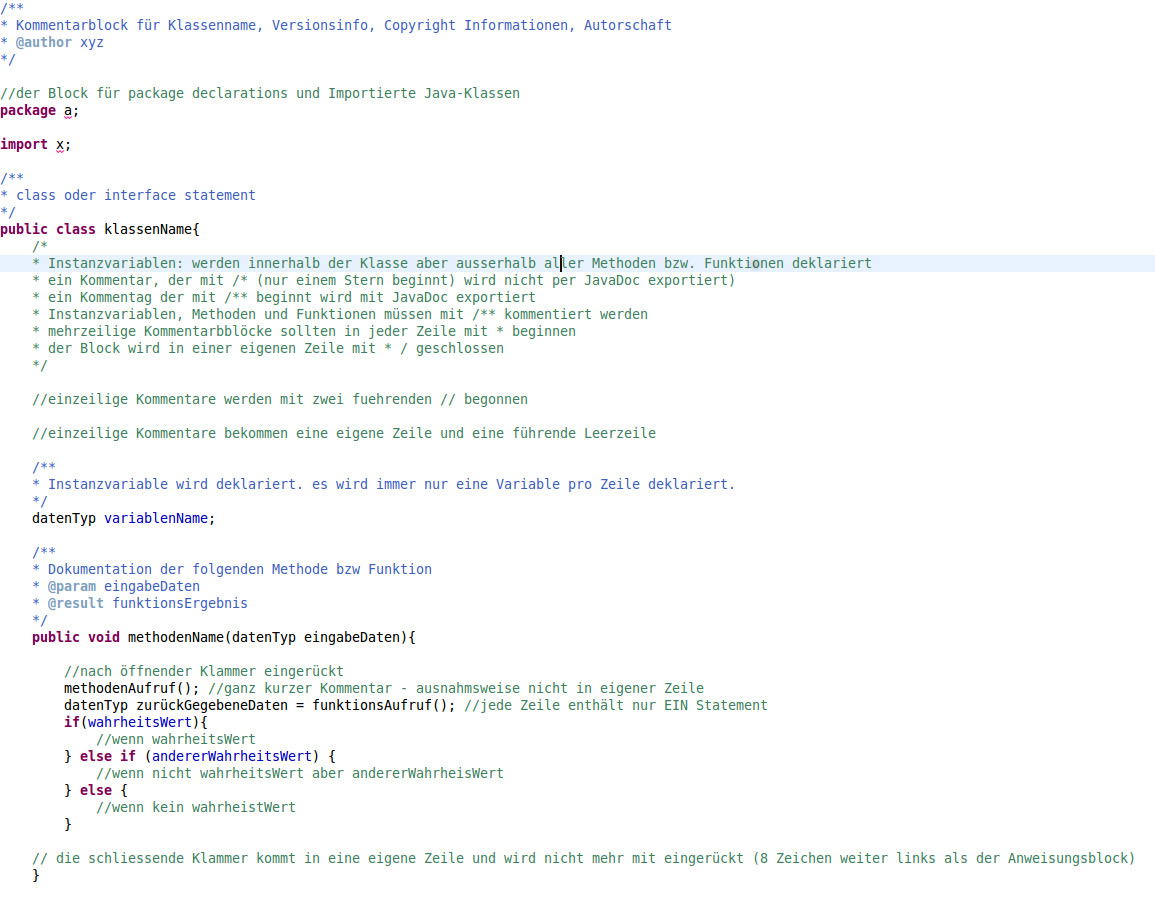
\includegraphics[scale=0.3]{Unbenannt.jpg}
%\caption{hier wird anhand von code gezeigt auf welchen Standard wir uns geeinigt haben}
  \label{PNFs}
\end{figure} 


%\subsection{Bespielcode}

\subsection{Testkonzept}

Zum Testen der einzelnen Klassen und Komponenten, kommt bei uns das Framework JUnit (für Java) bzw. JSUnit (für JavaScript) zum Einsatz. Da unser Ziel fehlerarmer Code ist, werden wir usneren Erzeugten Code laufend prüfen um auf etwaige Fehler immer schnellstmöglich aufmerksam zu werden. 
Die folgende geneuere Erklaerung für JUnit gilt analog so auch für JSUnit.
Da JUnit komplett in Java geschrieben ist, kann es alle sprachspezifischen Aspekte testen. Ein weiterer Vorteil von JUnit liegt darin, dass ein ausgereiftes Plug-in für die allermeisten bekannten IDEs existiert. Funktionsweise der Testumgebung: Es wird eine Funktion geschrieben, die einen Test auslöst. Dieser Test ist entweder grün oder rot. Sollte der Test rot sein, wird der auslösende Fehler genauestmöglich angezeigt. Diese Tests kann man manuell auslösen, oder in bestimmten Intervallen oder nach bestimmten Änderungen auslösen. So stellen wir sicher dass nichts implementiert wird, was nicht auch getestet ist. Während des Programmierens sollten die Fehler und die Fehlerbehandlung dokumentiert werden.
Im späteren Verlauf, sobald das Spiel lauffähig ist, müssen Tests derart durchgeführt werden, dass tatsächliches Spielen simuliert wird. Die dabei gefundenen Fehler werden dokumentiert. Der Tester führt darüber Protokoll welche Fehler auftreten. Ein Fehlerbehandler wird die Fehler im Programmcode suchen und behandeln. Die Fehlerbehandlung sollte ebenfalls dokumentiert werden, damit der nächste identische Fehler schneller behandelt werden kann. 

\subsection{Organisatorische Festlegungen}

Es findet jede Woche Donnerstags um 11 Uhr ein Teamtreffen mit dem Auftraggeber und Betreuer statt. Dabei analysieren wir die aktuellen Aufgabenstellungen, verteilen die Aufagben auf die Teammitglieder und haben die Möglichkeit mit dem Auftraggeber und/oder dem Betreuer Rücksprache zu halten. Nach Bedarf halten wir außerhalb dieser Treffen weitere Meetings ab um offene Fragen zu klären oder gemeinsam an Aufagben zu arbeiten. Die Koordination der Aufgaben organisieren wir mit Hilfe von trello (\url{https://trello.com/b/O1FKsQ6W/homepage}). Die Kommunikation untereinander läuft ebenfalls über trello sowie per xmpp-chat und per Mail. Dokumente an denen wir arbeiten, erstellen wir per PiratePad, so dass jedes Teammitglied jederzeit sieht wie der Fortschirtt ist, und jeder mithelfen kann einzelne Dokumente zu erstellen. Vorteilhaft an dieser Methode ist weiterhin, die dezentrale Speicherung der Dokumente. Der Quelltext den wir erstellen, wird per dezentralem Versionsverwaltungssystem git gespeichert und verteilt. Das hilft auch bei der Überprüfung der einzuhaltenden Coding-Standards und Dokumentatiosanforderungen.

\section{Glossar}
siehe externes Dokument
\end{document}